\documentclass[lecture.tex]{subfiles}

\begin{document}

\exercice{}
\video{https://youtu.be/Bw5OJeDmmE4}
\enonce{rdm-0038}{}


\begin{center}
  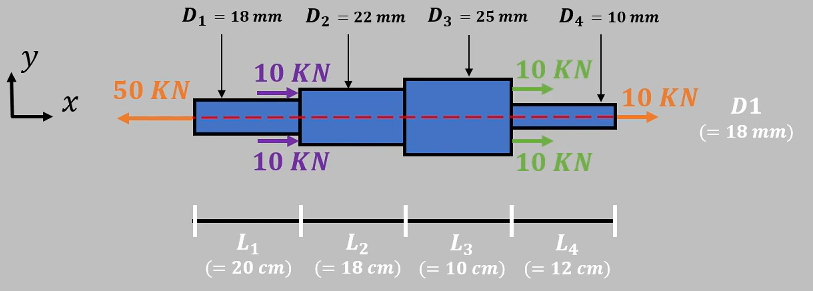
\includegraphics[scale=0.5]{figA0038.png}
\end{center}

\begin{enumerate}
  \item Tracer le diagramme de $N_{x}$ tout au lang de la barre.
  \item Tracer le diagramme de $\sigma_{N}$ tout au long de la barre.
  \item Vérifier la résistance de la barre si la contrainte $\sigma_{a d m}=14 \mathrm{kN} / \mathrm{cm}^{2}$.
  \item Calculer l'allongement ou le raccourcissement de la barre.
  \item En déduire le pourcentage de l'allongement et le pourcentage du raccourcissement dans la barre.

\end{enumerate}

\finenonce{rdm-0038}
\finexercice


\end{document}
